\documentclass[english,11pt]{report}		


%_____________________________________________________________________________
\usepackage[utf8]{inputenc}
\usepackage[T1]{fontenc}
\usepackage{geometry}
\usepackage[francais]{babel}
\usepackage{graphicx}
\usepackage{verbatim}
\usepackage{graphicx}
\usepackage{enumitem}
\usepackage{pifont}
\usepackage{multicol}
\usepackage{tikz}
\usepackage{pdfpages}
 
\graphicspath{{images/}}
%_____________________________________________________________________________

%_____________________________________________________________________________
\begin{document}
%_____________________________________________________________________________
\begin{titlepage}
	\centering
	%
\includegraphics[width=0.15\textwidth]{you}\par\vspace{1cm}
	
\includegraphics[width=0.15\textwidth]{univ}\par\vspace{1cm}
	{\scshape\LARGE Université de Montpellier \par}
	\vspace{1cm}
	{\scshape\Large Rapport pour le TER\par}
	\vspace{1.5cm}
	{\huge\bfseries Sokoban\par}
	\vspace{2cm}
	{\Large Paola \textsc{Andreu}, Yanis \textsc{Bled}, Thiziri \textsc{Harcheb}, Aurélie \textsc{Murcia}, Marine \textsc{Pellicer}, Julien \textsc{Roussé}}

	\vfill
	
	{\Large Supervisé par\par}
	\vspace{0.2cm}
	{\Large Violaine \textsc{Prince}}
	
	\vfill


	{\large \today\par}
\end{titlepage}


\tableofcontents
%_____________________________________________________________________________


%_____________________________________________________________________________
\chapter*{Introduction}
%_____________________________________________________________________________

L’objet de ce rapport est de présenter synthétiquement le travail réalisé dans le cadre du TER. Le projet que nous avons choisi porte sur le jeu de Sokoban. Notre but était d’améliorer une version existante de ce jeu \cite{sokoban}.\par
\vspace{0,5cm}
Le principe du Sokoban est de diriger un personnage dans un labyrinthe. Ce personnage doit pousser les caisses jusqu'aux objectifs indiqués sur la carte. La partie est gagnée lorsque le joueur a placé toutes les caisses sur leurs cibles.\\ Pour commencer, afin d'identifier les points positifs, négatifs et les limites de la version de base, il nous a fallu faire preuve d'esprit critique. Ensuite, à partir de l'ensemble des améliorations proposées au sein du groupe, nous avons construit le cahier des charges que nous avons essayé de respecter tout au long du projet. Aujourd’hui, nous pouvons dire que le cahier des charges a été respecté et que les améliorations que nous souhaitions apporter au projet ont été réalisées.\\
Nous nous sommes répartis le travail afin que chacun ait une partie à traiter et à présenter à chaque réunion (dont les comptes rendus sont disponibles en annexe). Nous avons désigné un chef de projet afin d’organiser les réunions et d’établir un lien avec notre tutrice. Au fur et à mesure des avancées, chacun de nous a donné son avis et a apporté ses connaissances pour faire progresser le projet.\\
Nous avons donc amélioré le jeu Sokoban afin qu’il propose plus de fonctionnalités. Nous avons changé l’interface du jeu, étoffé et corrigé l’éditeur, ajouté un système de score et créé des niveaux progressifs. Sur un plan technique, nous avons programmé en C/C++, ce qui nous a permis d’approfondir nos connaissances, en plus de découvrir de nouvelles possibilités de programmation.\\
Nous nous sommes aussi servis de la bibliothèque SDL \cite{SDL}, qui était la bibliothèque proposée dans la version d’origine. Son utilisation nous a permis de nous initier à la programmation multimédia en deux dimensions. En l’occurrence, nous avons appris à gérer les évènements, l’affichage et la gestion des périphériques ; ceci sera plus amplement détaillé dans la suite du rapport.\par
\vspace{0,5cm}
Après avoir présenté le cahier des charges de notre projet, nous expliquerons les choix effectués durant celui-ci. Nous exposerons également les problèmes rencontrés, et nous terminerons par une brève conclusion qui portera sur le parcours qu'a fait notre projet.

%_____________________________________________________________________________
\chapter{Gestion du projet}
%_____________________________________________________________________________

Ce projet est une opportunité pour apprendre à travailler en équipe. La nôtre est constituée de 6 étudiants. Nous avons collectivement analysé la version existante du jeu et rédigé notre cahier des charges en conséquence. Au regard de la structure que présentait la version initiale du jeu, nous avons décomposé le projet en 3 grandes parties :\par
\vspace{0,1cm}
\begin{itemize}
    \item{l'éditeur de carte}
    \item{le jeu}
    \item{le tableau de bord}
\end{itemize}\par
\vspace{0,1cm}
Nous avons réparti le groupe sur ces 3 parties en prenant en compte leur complexité. Ainsi Paola Andreu, Marine Pellicer et Thiziri Harcheb ont travaillé sur le jeu, Aurélie Murcia et Julien Roussé sur le menu et l’éditeur de cartes et Yanis Bled sur le tableau de bord. Nous avons également désigné un chef de projet afin de faciliter la mise en commun des différentes contributions.\par
\vspace{0,5cm}
Sur un plan organisationnel, nous avons décidé de faire une réunion bilan toutes les semaines afin de déterminer où en étaient les objectifs et si des problèmes s'étaient posés durant l'avancée des différentes parties.\par
\vspace{0,1cm}
Sur un plan technique, nous avons utilisé plusieurs outils informatiques afin de gérer le projet. En ce qui concerne la programmation, nous avons retenu l’outil de versioning \emph{Git} \cite{gitlab}. Il nous a permis de mettre en commun et gérer plus aisément les différentes versions apportées par nos contributions. Nous avons de plus échangé des informations par l’intermédiaire d’outils classiques, comme la messagerie électronique ainsi que la messagerie instantanée Facebook (chat).\par
\vspace{0,5cm}
\textbf{Qu'est-ce que la bibliothèque SDL ?}
\vspace{0,15cm}
\begin{itemize}[label=\ding{223}]
    \item {La bibliothèque SDL est une bibliothèque de bas niveau particulièrement utilisée pour créer des jeux en 2D. Il s’agit d’une bibliothèque tierce, c’est-à-dire qu’elle n’est pas initialement installée sur l'ordinateur. Il faut donc la télécharger et l’installer avant de pouvoir l’utiliser. Comme elle est écrite en C,  elle peut être utilisée par des programmes en C, C++ (mais existe également en Java). C’est une bibliothèque libre et gratuite, multi-platforme.\\Pour notre projet Sokoban, nous avons utilisé la SDL pour la création de fenêtres, la gestion des images, du son et du temps. En effet, la bibliothèque SDL permet de créer des fenêtres de la dimension souhaitée, elle permet également d’affecter une image donnée à une partie de la fenêtre créée en spécifiant les coordonnées (en pixels) de l’endroit où on souhaite voir l’image.\\Cette bibliothèque a également des fonctions permettant d’effectuer des actions lors d’un évènement. Un \emph{évènement}  a lieu quand l'utilisateur appuie sur une touche du clavier, quand il clique avec la souris, quand il bouge la souris, quand il réduit la fenêtre, quand il demande à fermer la fenêtre... Elle prend donc en charge la gestion du clavier et de la souris.}
\end{itemize}
\vspace{0,5cm}
\textit{Tous les développements ont été réalisés en C/C++ avec \emph{gpp} comme compilateur. }

%_____________________________________________________________________________
\chapter{Cahier des charges}
%_____________________________________________________________________________

Dans cette partie nous allons présenter les différents objectifs que nous nous sommes fixés au début du projet.\par
Tout d'abord, voici quelques captures de la version sur laquelle nous avons travaillé :\par
\vspace{0.2cm}
\begin{itemize}[label=\ding{71}]
    \item{\textbf{Voici l'écran d'accueil :}}
\end{itemize}
\vspace{0.2cm}
%
\begin{center} 
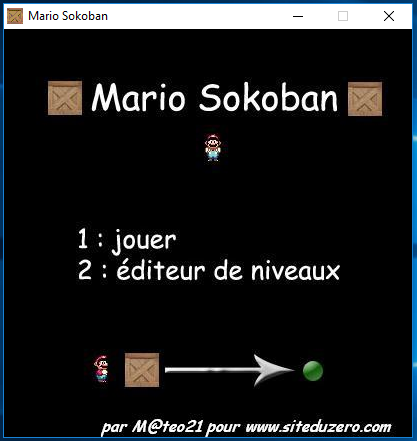
\includegraphics[scale=0.75]{menuO}
\end{center}
%
\vspace{0.2cm}
\begin{itemize}[label=\ding{71}]
    \item{\textbf{Voici l'écran de jeu :}}
\end{itemize}
\vspace{0.2cm}
%
\begin{center} 
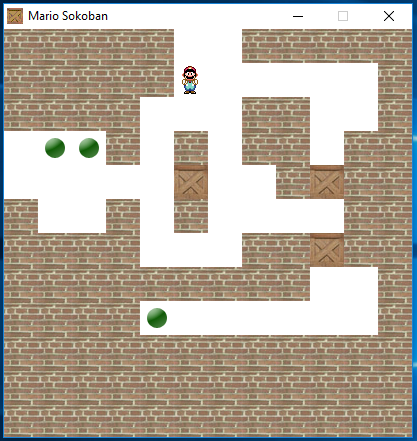
\includegraphics[scale=0.75]{jeuO}
\end{center}
%
\vspace{0.2cm}
\begin{itemize}[label=\ding{71}]
    \item{\textbf{Voici l'écran de l'éditeur :}}
\end{itemize}
\vspace{0.2cm}
%
\begin{center} 
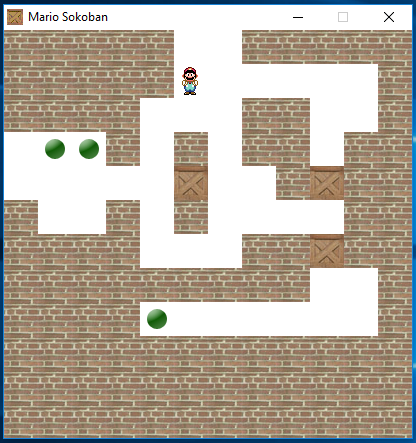
\includegraphics[scale=0.75]{editeurO}
\end{center}
\vspace{0.5cm}
\textit{(Comme vous pouvez le constater, sur la version de départ, l'éditeur et le jeu sont identiques en tous points)}\par
\vspace{0.2cm}
Étant donné que le projet visait à améliorer les différents aspects du jeu, le cahier des charges peut être divisé selon plusieurs domaines, à savoir :\par
\vspace{0,1cm}
\begin{itemize}[label=\textbullet]
    \item{"Jouabilité ":}
    \begin{itemize}
        \item{créer un système de niveaux progressifs : dès que l’on réussit un niveau, le jeu enchaîne sur le niveau suivant}
        \item{améliorer la facilité d’utilisation du jeu, son ergonomie, notamment avec des graphismes de meilleure qualité}
        \item{proposer les touches « retour » et « recommencer »}
        \item{ajouter la possibilité de charger une sauvegarde}
        \item{placer les cartes créées dans l'éditeur de carte dans un niveau « personnalisé »}
        \item{faire en sorte que le jeu puisse tourner en même temps que d’autres applications en améliorant les performances}
    \end{itemize}
    \item{Fonctionnalités :}
    \begin{itemize}
        \item{créer un mode d’emploi avec une aide ergonomique}
        \item{prendre en charge la gestion de la souris}
        \item{mettre en place un compteur de temps}
        \item{en se basant sur le temps, installer un système de score}
        \item{permettre au joueur de s'identifier et enregistrer ses scores}
        \item{faire des vérifications avant de valider une carte créée dans l’éditeur}
        \item{proposer un menu \textbf{options} (couper le son, changement des touches)}
        \item{gérer des bonus/malus en fonction du temps mis à résoudre une carte}
        \item{proposer des indices si le joueur bloque (avec possibilité de malus sur le score final)}
        \item{ajout d’une bande son}
        \item{ajout d’un choix pour la difficulté}
    \end{itemize}
    \item{Graphismes :}
    \begin{itemize}
        \item{rajouter un message de félicitations à la fin de chaque partie gagnée}
        \item{mise en place d’un tableau de bord intuitif}
        \item{mise en place d’un menu « Accueil »}
    \end{itemize}
\end{itemize}

%_____________________________________________________________________________ 
\chapter{Choix effectués}
%_____________________________________________________________________________

Comme vous avez pu le constater, de nombreuses améliorations et changements étaient nécessaires, nous allons dans cette partie vous décrire ce que nous avons mis en œuvre et pourquoi.\par
\vspace{0,5cm}
Dès le lancement du jeu, nous avons choisi d’animer une petite introduction, ce n’est pas un choix anodin. En effet, nous n’avons finalement pas fait de tutoriel, le jeu étant simpliste et relativement intuitif. Nous avons donc décidé de faire cette petite animation en introduction qui reprend le principe du jeu : un personnage déplace une caisse vers un objectif. Nous voulions ainsi donner un avant-goût du jeu et en rappeler le principe.\par
\vspace{0,2cm}
Passé l’introduction, nous arrivons sur l’écran d’accueil. Musique calme et design minimaliste ont été choisis ici pour mettre le joueur dans une ambiance de réflexion. D’ailleurs le design minimaliste, très épuré, a été choisi très tôt dans le projet pour suivre l’idée de rendre le jeu intuitif et agréable pour l’utilisateur.\par
\vspace{0,2cm}
À la base, nous voulions permettre à un joueur de s’identifier dès le début du jeu. Le problème est qu’il aurait alors fallu stocker toutes les données de tous les utilisateurs et leurs cartes personnalisées. C’est pourquoi nous avons décidé de ne demander le nom de l’utilisateur que si celui-ci faisait un nouveau meilleur score. De plus, mettre les cartes personnalisées en commun permet également de rajouter du contenu, et il est intéressant de pouvoir jeter un œil sur les créations des autres joueurs.\par
\vspace{0,2cm}
Puisque la bibliothèque SDL que nous avons utilisée ne permet pas de créer des boutons, nous avons dû utiliser une image pour indiquer à l’utilisateur quel choix était sélectionné (par défaut sur Jouer).\par
\begin{center} 
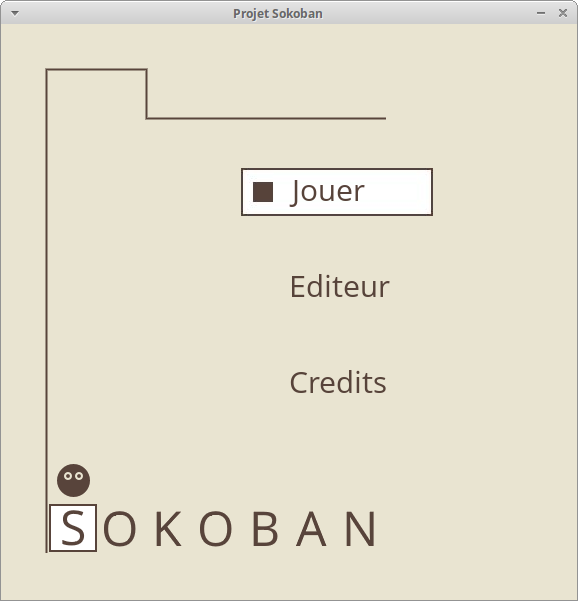
\includegraphics[scale=0.4]{menu}
\end{center}
\par
Nous avons, par souci d’ergonomie, rendu possible de naviguer dans le menu avec la souris aussi bien qu’avec les touches directionnelles. Il en va de même pour le reste du jeu.\par
\vspace{0,2cm}
Comme le jeu propose deux fonctionnalités qui sont l’éditeur (permettant de créer des cartes), et le jeu en lui-même, nous avons fait le choix d’un modèle hiérarchisé. C’est donc à partir du menu que l’on accède au jeu et à l’éditeur.\par
\vspace{0,2cm}
Nous allons détailler chaque améliorations apportées à ces deux aspects, séparément, et en commençant par la partie qui concerne le jeu Sokoban en lui-même.\par
\clearpage
\vspace{0.5cm}
\begin{itemize}[label=\ding{71}]
    \item{\textbf{Dans le jeu :}}
\end{itemize}
\vspace{0.5cm}
\begin{center} 
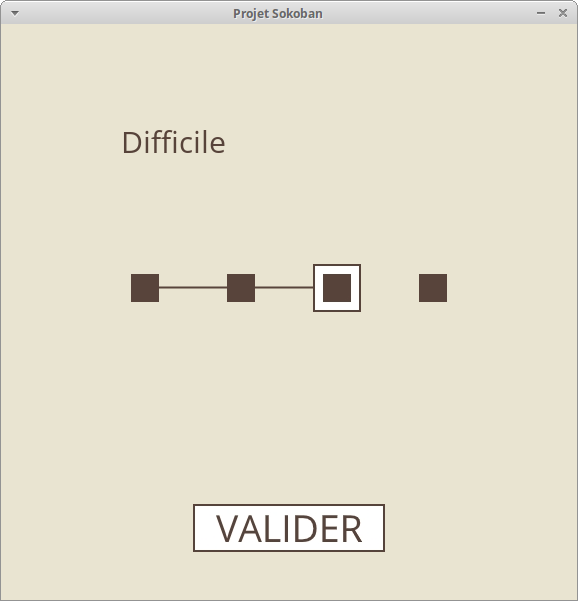
\includegraphics[scale=0.4]{difficultes}\par
\end{center}
\par
Si le joueur lance une partie, nous lui proposons d’abord de choisir le niveau de difficulté entre Facile, Normal, Difficile et Personnalisé – dans lequel il peut retrouver toutes les cartes créées via l’éditeur (sujet que nous aborderons par la suite).\par
\vspace{0.2cm}
Une fois le niveau de difficulté choisi, nous proposons à l’utilisateur de sélectionner une carte parmi les 10 qui sont proposées par défaut pour chacun des niveaux de difficulté.\par
\vspace{0.5cm}
\begin{center} 
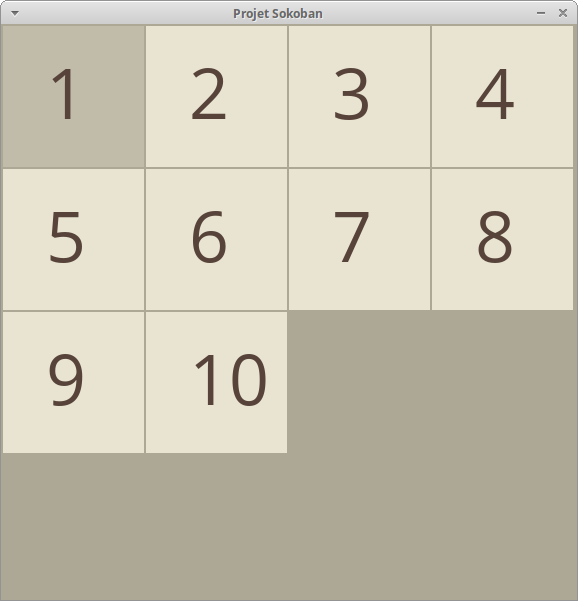
\includegraphics[scale=0.4]{cartes}
\end{center}
\vspace{0.2cm}
\vspace{0.2cm}
Une fois le niveau et la carte choisis nous voilà donc en jeu.\par
\vspace{0.5cm}
\begin{center}
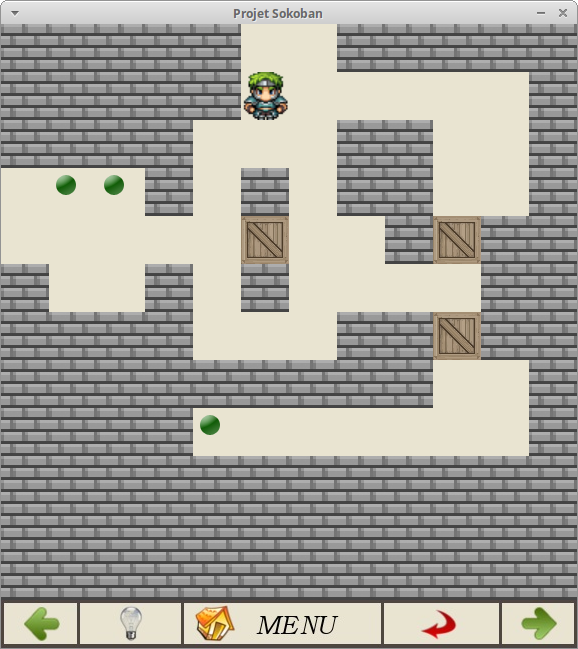
\includegraphics[scale=0.4]{jeu}
\end{center}
\vspace{0.2cm}
\par
Comme vous pouvez le voir, le jeu se démarque à présent de la version d’origine. En effet nous avons remplacé le décor pour le rendre plus « moderne », mais surtout pour pouvoir agrandir la taille de la fenêtre. Comme expliqué dans le cahier des charges ; dans la version d’origine, il était impossible de redimensionner la fenêtre qui était par défaut très petite.\par
\vspace{0.2cm}
Nous nous sommes rendus compte que c’était dû à la bibliothèque SDL, et surtout à l’utilisation d’images fixes. Redimensionner la fenêtre aurait changé la taille des images et donc détruit totalement le rendu souhaité. Notre version ne permet pas non plus de redimensionner la fenêtre, mais nous avons toutefois augmenté la taille des sprites (48x48 pixels) et donc la taille de la fenêtre.\par
\vspace{0.2cm}
Ensuite, par soucis de faciliter l’accès aux nouvelles fonctionnalités, nous avons ajouté un tableau de bord. Le tableau de bord est spécifique selon s’il se trouve dans l’éditeur ou dans le jeu.\par
\vspace{0.5cm}
\begin{center}

\includegraphics[scale=0.8]{tableau}
\end{center}
\vspace{0.2cm}
\par
Dans le jeu, le tableau de bord possède une flèche à chacune de ses extrémités. Elles permettent de naviguer entre les cartes ; celle de gauche donne sur la précédente, celle de droite sur la suivante.\par
\vspace{0.2cm}
La flèche rouge permet d’annuler le dernier déplacement effectué par le joueur et de revenir ainsi jusqu’au début. Si nous avons décidé d’offrir au joueur la possibilité de revenir en arrière, c'est parce qu'il suffit qu'une caisse soit bloquée pour qu'il n’y ait plus moyen de continuer. Dans la version que nous avons testée, il fallait alors quitter la carte et la recharger, ce qui devenait rapidement fastidieux.\par
\vspace{0.2cm}
Cette fonctionnalité a été longuement discutée, nous pensions au début mettre un message d’échec si le joueur bloquait toutes ses caisses, mais nous avons rapidement compris que cela pouvait rendre le jeu frustrant car dans certains niveaux, il faut essayer plusieurs fois avant de trouver la solution. Nous avons donc opté pour une fonction retour.\par
\vspace{0.2cm}
L’icône d’ampoule quant à elle, permet d’afficher la liste des commandes, c’est une petite aide pour les joueurs novices qui ne seraient familier avec les jeux vidéos.\par
\vspace{0.2cm}
Enfin en passant le curseur sur l’icône menu, un menu déroulant offre le choix entre recommencer la carte actuelle, revenir à l’écran d’accueil ou voir les crédits du jeu.\par
\vspace{0.5cm}
\begin{center}
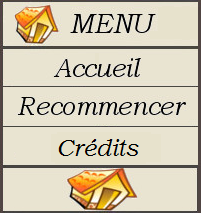
\includegraphics[scale=0.8]{MenuD}
\end{center}
\vspace{0.2cm}
\par
Lors du test du jeu d’origine, nous nous sommes rendu compte que le jeu n’était pas adapté à tous les claviers. En effet, ceux ne possédant pas de pavé numérique étaient incapables d’accéder au jeu. C’est pour cette raison que nous avons rendu l’intégralité de la navigation dans le jeu possible à la souris ou au clavier. Ainsi, le joueur peut utiliser sa souris pour accéder au jeu, créer les cartes dans l’éditeur…\par
\vspace{0.2cm}
Seul le déplacement du personnage se fait uniquement avec les touches directionnelles. En effet, nous ne permettons pas de jouer avec la souris car, si le joueur désigne une position où le personnage doit se déplacer à l’aide de la souris, celui-ci va alors se téléporter à cet emplacement, ce qui rend impossible la gestion des caisses.\par
\vspace{0.5cm}
\begin{center}
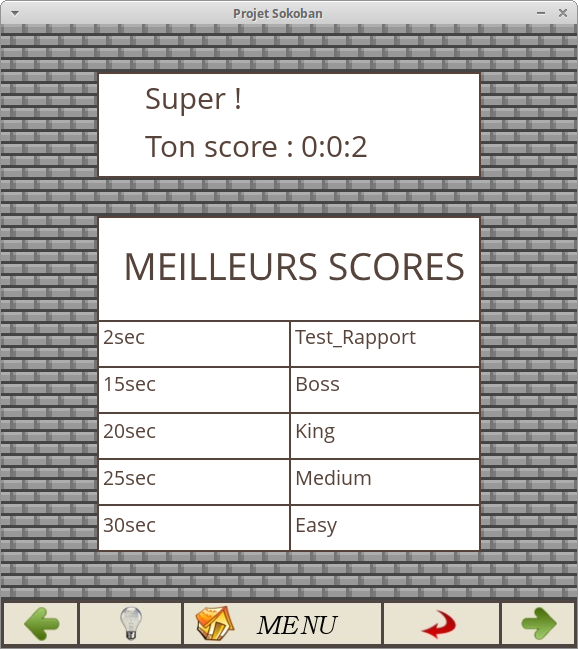
\includegraphics[scale=0.4]{score}
\end{center}
\vspace{0.2cm}
\par
Enfin, afin d’ajouter un peu de compétitivité entre les différents joueurs, nous avons instauré un système de score. Celui-ci est basé sur le temps mis pour finir la carte. Pour chaque carte, les cinq meilleurs joueurs sont enregistrés dans un fichier texte à part, que le jeu va lire. Si le score est meilleur que ceux sauvegardés, alors le joueur a la possibilité d’entrer son nom directement dans le jeu.\par
\vspace{0.5cm}
\begin{itemize}[label=\ding{71}]
    \item{\textbf{Dans l'éditeur :}}
\end{itemize}
\vspace{0.5cm}
\begin{center}
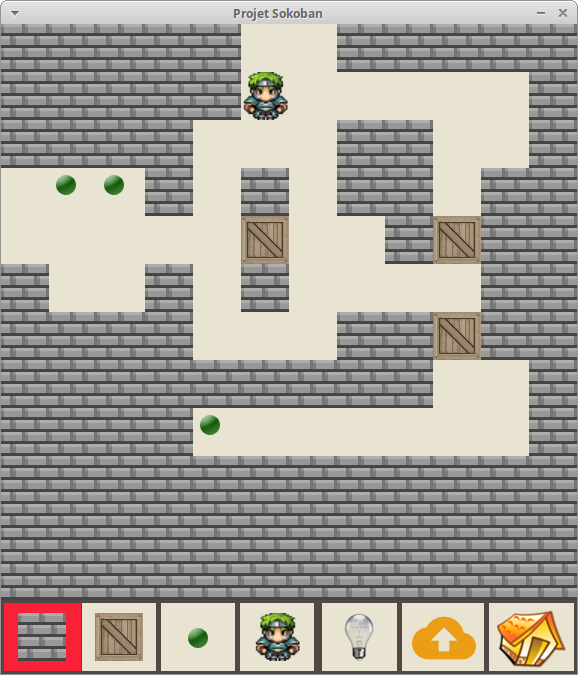
\includegraphics[scale=0.4]{editeur}
\end{center}
\vspace{0.2cm}
\par
Pour continuer avec l’éditeur, il a fallu corriger plusieurs problèmes avant de penser à ajouter des fonctionnalités. Premièrement, un bug permettait au joueur de poser plusieurs fois le personnage sur la carte. Deuxièmement, il pouvait créer des cartes inexploitables, avec un nombre d’objectifs différent du nombre de caisses. Pour résoudre le problème, nous empêchons la sauvegarde de la carte tant que le nombre de caisse(s) et le nombre d’objectif(s) ne sont pas égaux, et nous affichons un message d’erreur sur l’écran pour prévenir le joueur.\par
\vspace{0.2cm}
Ensuite, dans la version améliorée du Sokoban, sauvegarder une carte l’enregistrait à la place de la première carte. Afin de permettre au joueur de créer autant de cartes qu’il le souhaite, nous avons décidé de les stoker dans un niveau à part, appelé « personnalisé ». Mais pour éviter le stockage de doublons, nous avons réutilisé le système de message d’erreur afin de prévenir le joueur s’il tente d’enregistrer une carte déjà existante (nous vérifions si elle n’existe pas déjà).\par
\vspace{0.2cm}
Nous avons aussi effectué un travail d’optimisation. En effet la façon dont était programmé l’éditeur dans le code original a rapidement posé problème. À chaque fois qu’un bloc était ajouté ou supprimé, chaque case de l’écran était réaffichée, ce qui provoquait rapidement des ralentissements. Nous avons donc changé cela pour que seule la case modifiée soit réactualisée.\par


%_____________________________________________________________________________ 
\chapter{Problèmes rencontrés}
%_____________________________________________________________________________

Lors du projet nous avons rencontré plusieurs problèmes dont trois \'etaient directement liés à la bibliothèque SDL elle-même et donc impossibles à résoudre. Tout d’abord, nous souhaitions permettre un affichage en plein écran, mais les images utilisées par SDL ont une taille fixe. Il devenait alors impossible de s’adapter aux différentes résolutions d’écran. À la place, nous avons donc légèrement amélioré la qualité des images et agrandi la fenêtre de jeu, tout en gardant une taille qui convienne pour tous.\par
\vspace{0.2cm}
Le deuxième problème posé par la bibliothèque SDL que nous avons utilisée vient du fait qu’elle n’est pas compatible avec toutes les souris. En effet, certaines fonctionnent très mal avec SDL et provoquent d’importants ralentissements (ce dont nous nous sommes rendus compte durant les tests de notre version).\par
\vspace{0.2cm}
Le troisième point est également lié à la souris et aux performances. Bien qu’il n’empêche pas le jeu en lui-même, il peut se révéler problématique pour des ordinateurs à faible capacité. En effet, la gestion de la souris avec SDL est catastrophique. À chaque déplacement, le processeur est utilisé à 25\%, ce qui est beaucoup trop gourmand en ressources.\par
\vspace{0.2cm}
Durant la programmation, nous avons également eut une incompatibilité de la fonction retour avec le score. En effet le score devait normalement s’afficher au cours du jeu mais ne s’actualisait que lorsque la souris ou le personnage étaient déplacés. L’alternative pour laquelle nous avons finalement optée est de ne montrer le temps réalisé qu’une fois la carte terminée.\par
\vspace{1cm}
Enfin, certains objectifs du cahier des charges n’ont pas été remplis. Notamment l’ajout d’une option qui aurait permis de changer la configuration des touches. En effet, cette proposition était censée palier au problème d’absence de pavé numérique, par exemple, ou des claviers qui ne disposaient pas de certaines touches. Mais la gestion de la souris a justement été ajoutée pour régler ce problème.\par
\vspace{0.2cm}
Le système d’indices pour guider le joueur a finalement été oublié, car combiné à l’avantage qu’offre la possibilité d’annuler un déplacement, il n’y aurait presque plus aucune difficulté au jeu et ce n’était pas ce que nous souhaitions.\par
\vspace{0.2cm}
L’idée de changer le décor en fonction du niveau de difficulté ne s’est pas concrétisée pour deux raisons. Déjà, le jeu gère beaucoup d’images (personnage, caisses, objectifs, fond, murs, menu, tableau de bord, …) et nous ne souhaitions pas l’alourdir plus. Ensuite, parce que trouver des images qui s’accorderaient entre elles dans les différents niveaux de difficulté était une tâche presque impossible, à moins de les créer nous-même.\par
\vspace{0.2cm}
Enfin, nous devions ajouter un bouton « quitter » dans le tableau de bord mais nous avons finalement corrigé le bug de la version originale avec lequel cliquer sur la croix ramenait au menu. À présent, cela ferme directement le jeu. Nous avons donc annulé le bouton quitter pour le remplacer par un retour à l’accueil.\par
\vspace{0.2cm}

\appendix
\chapter{Comptes rendus}
Voici les comptes rendus tenus au cours des différentes entrevues du TER :
\vspace{0.2cm}
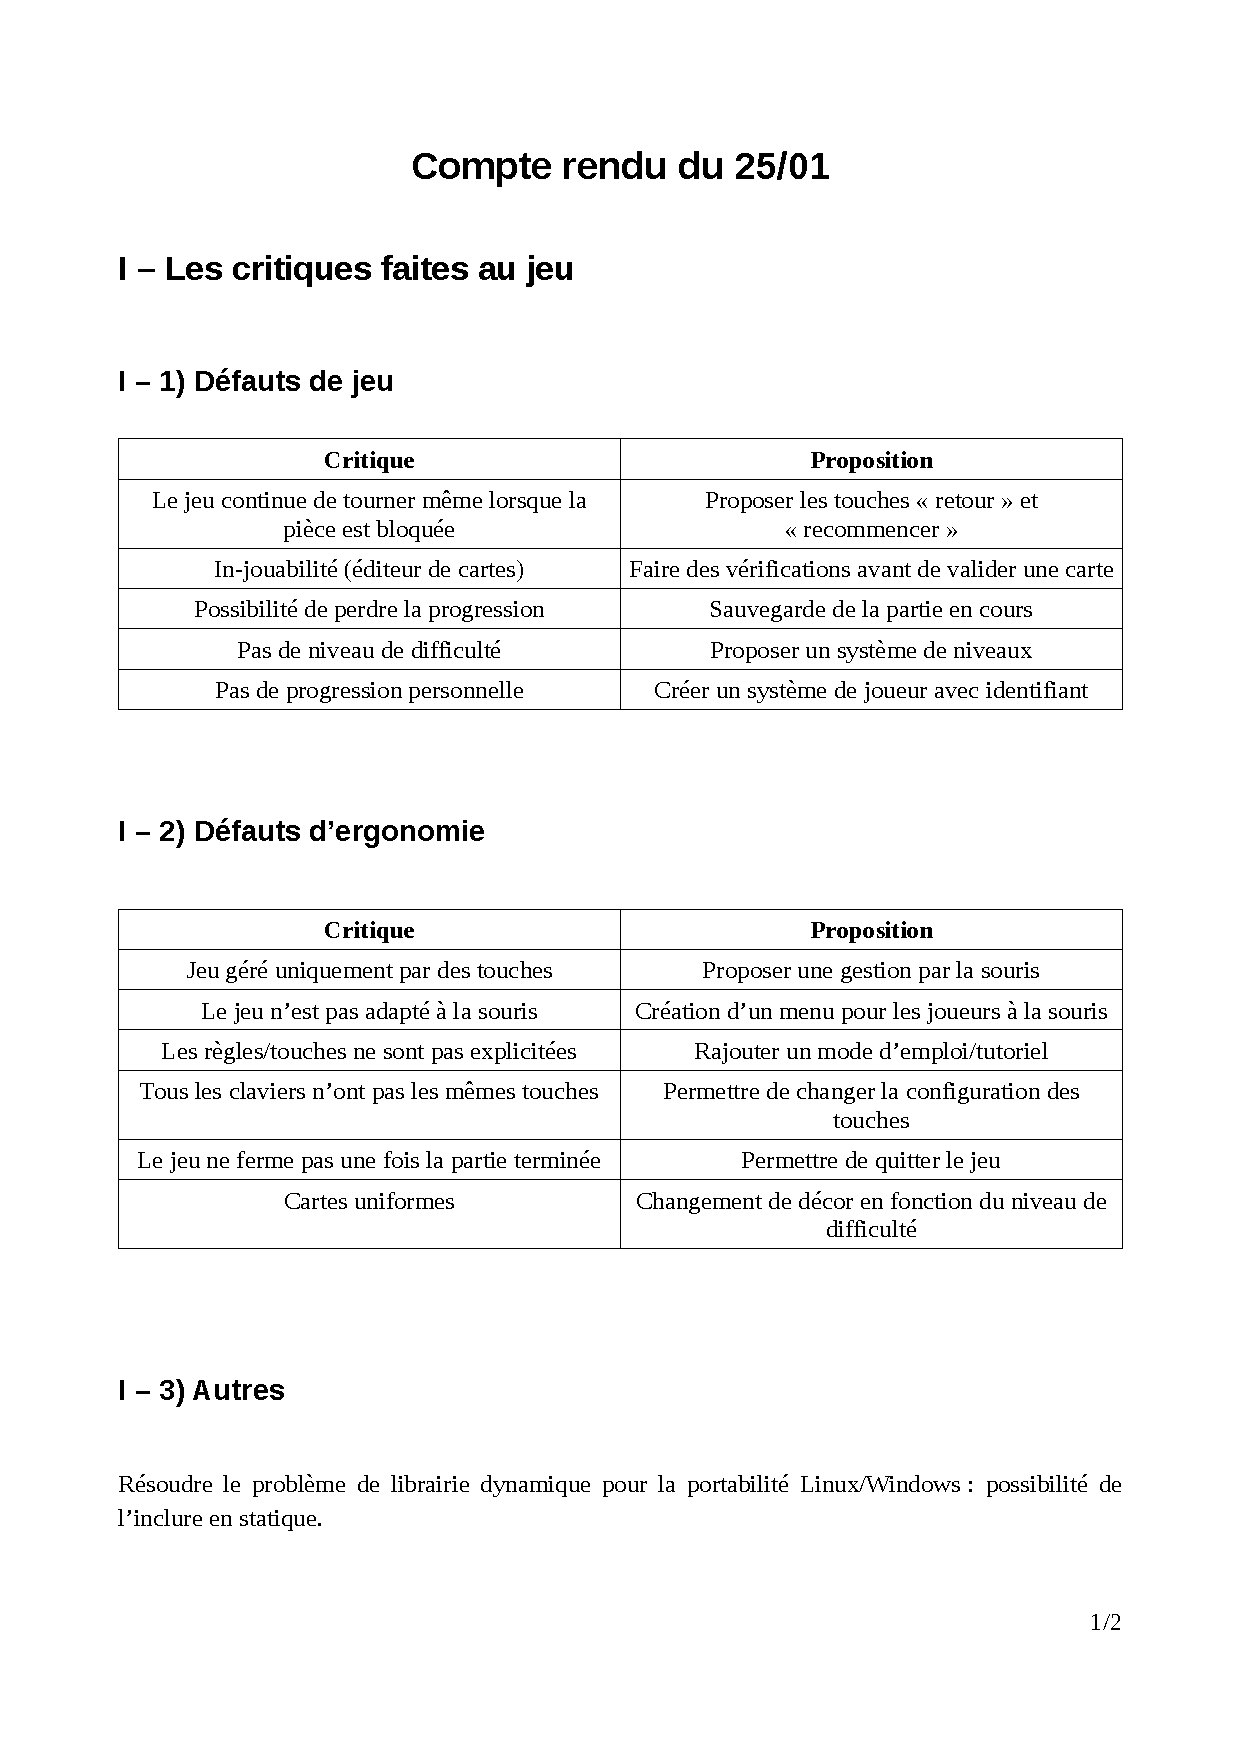
\includepdf[pages={1,2}]{CR1.pdf}
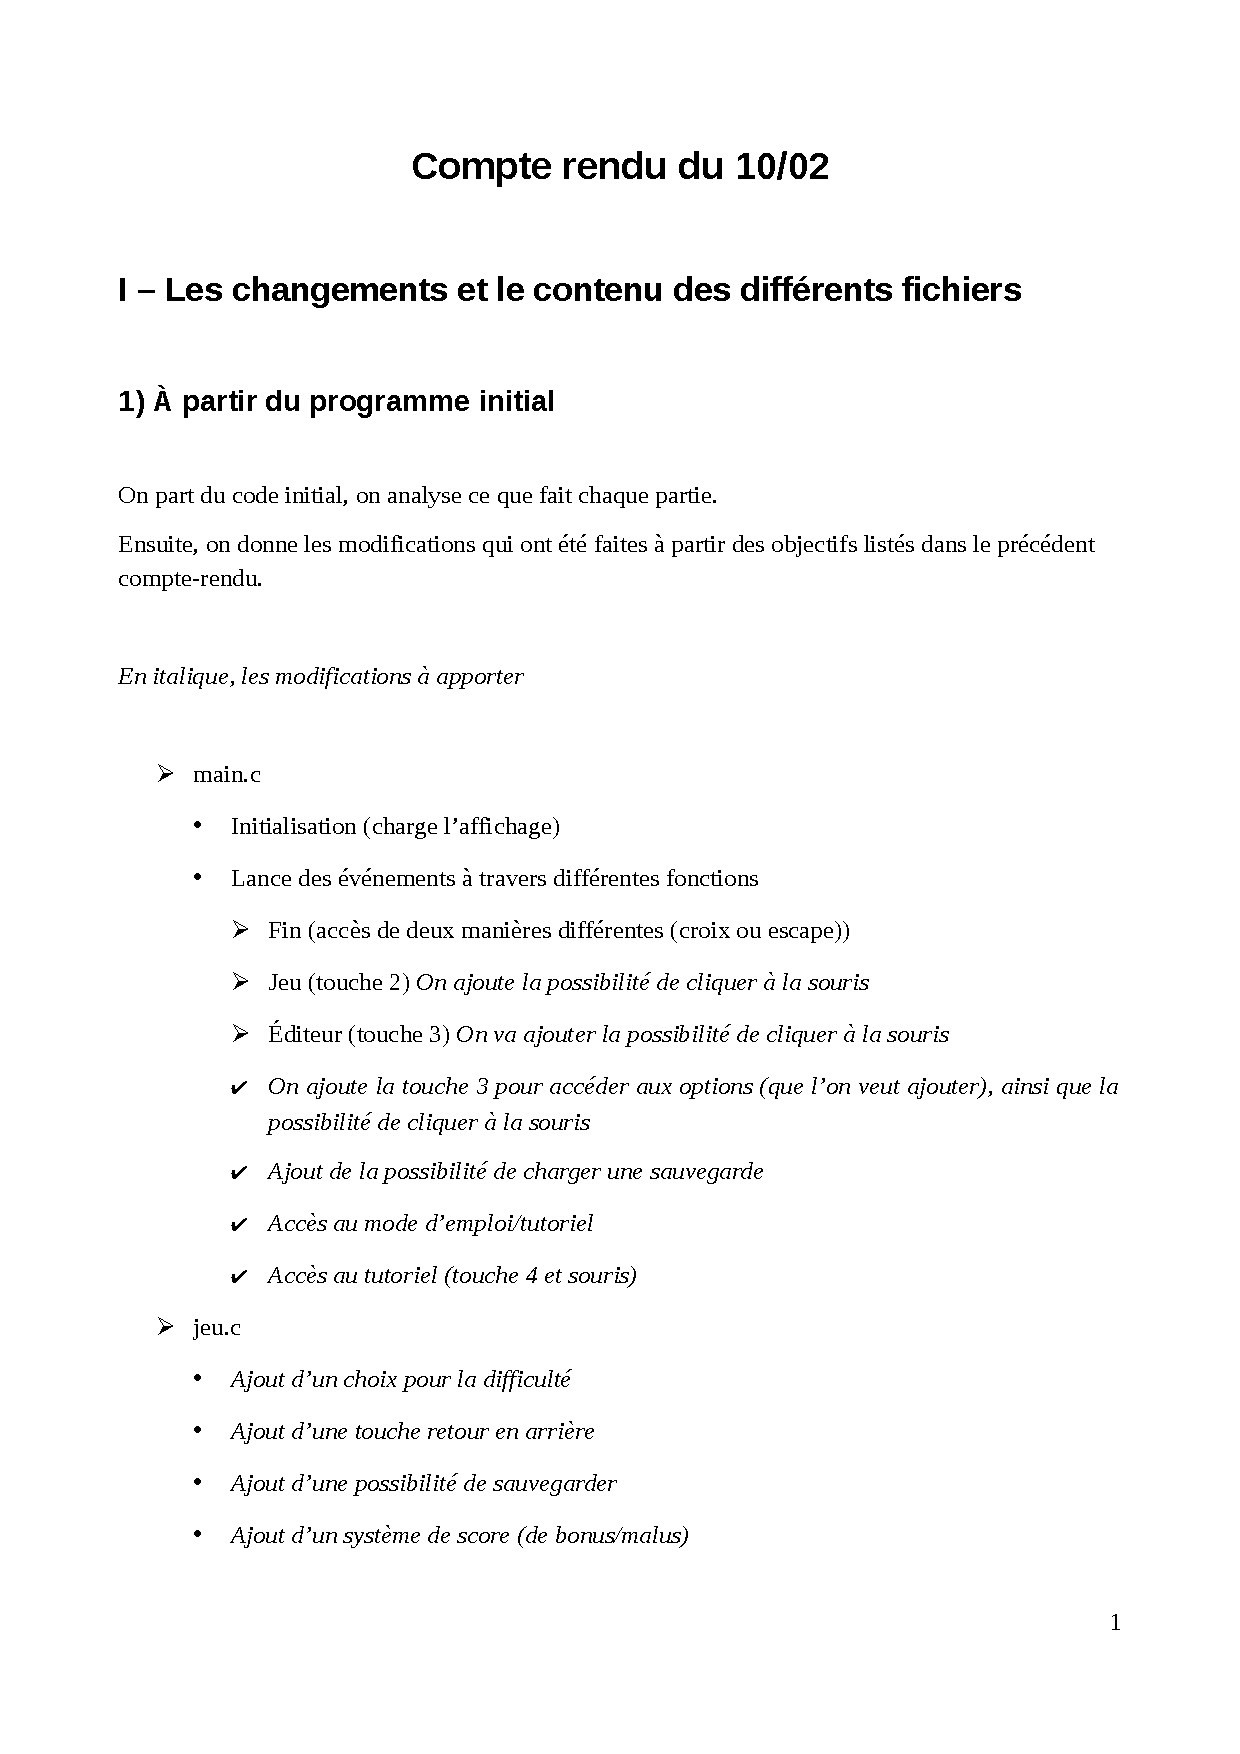
\includepdf[pages={1,2}]{CR2.pdf}
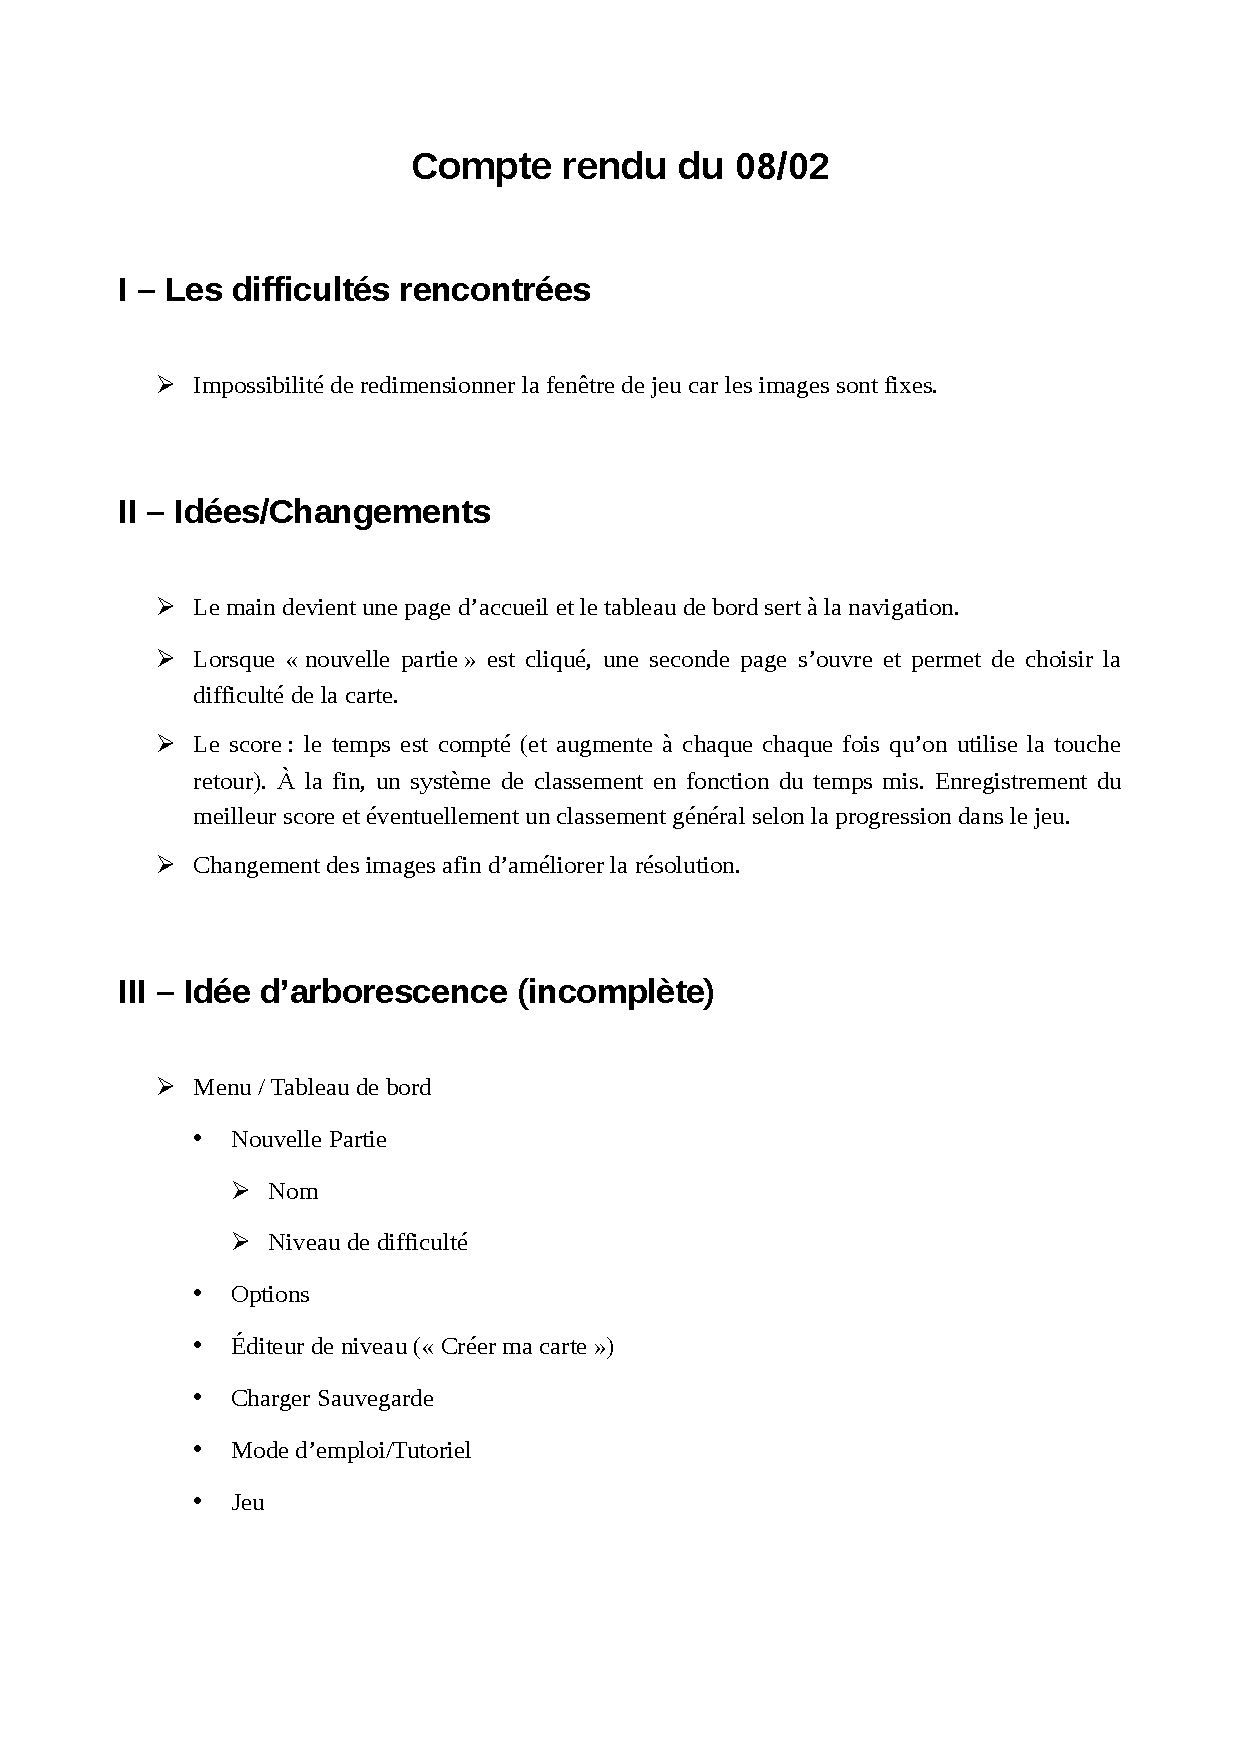
\includepdf[pages={1,2}]{CR3.pdf}
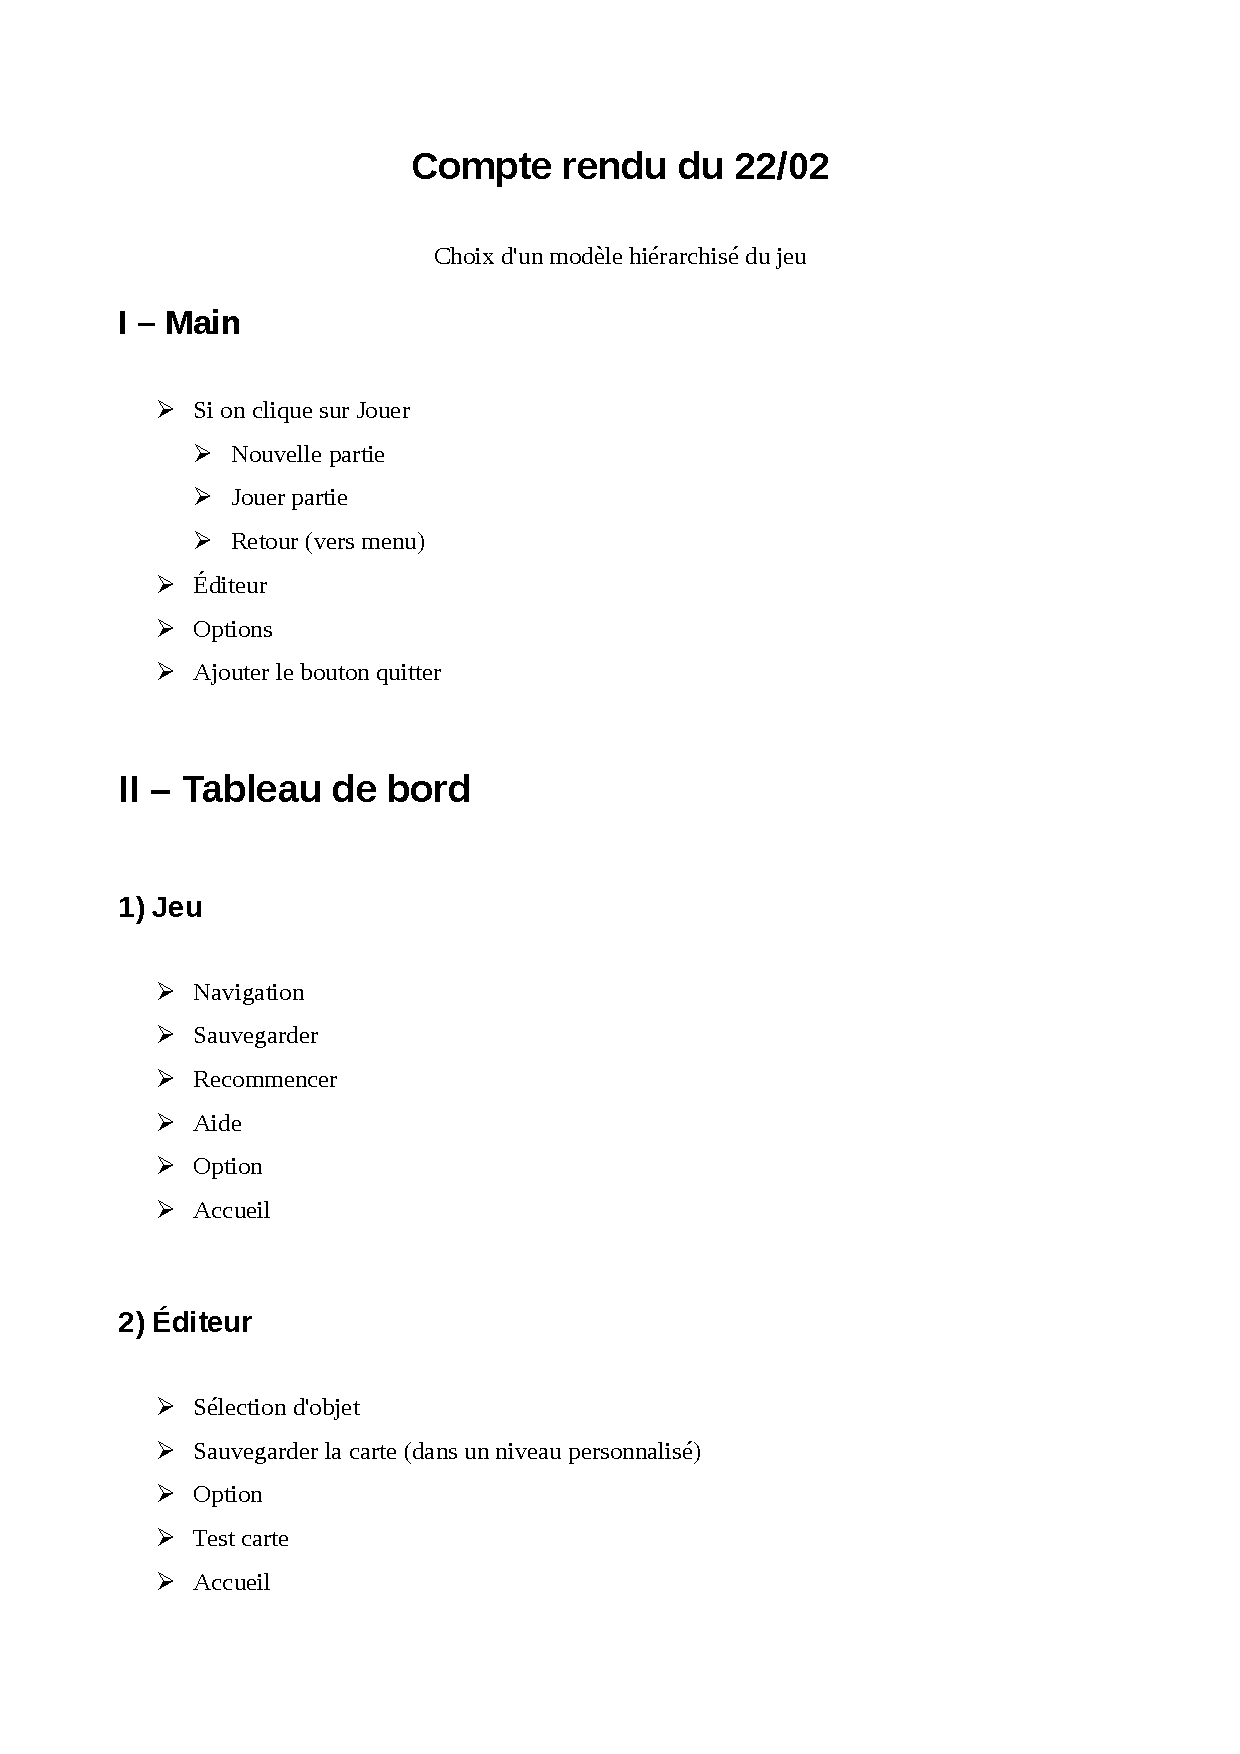
\includepdf[pages={1,2,3}]{CR4.pdf}
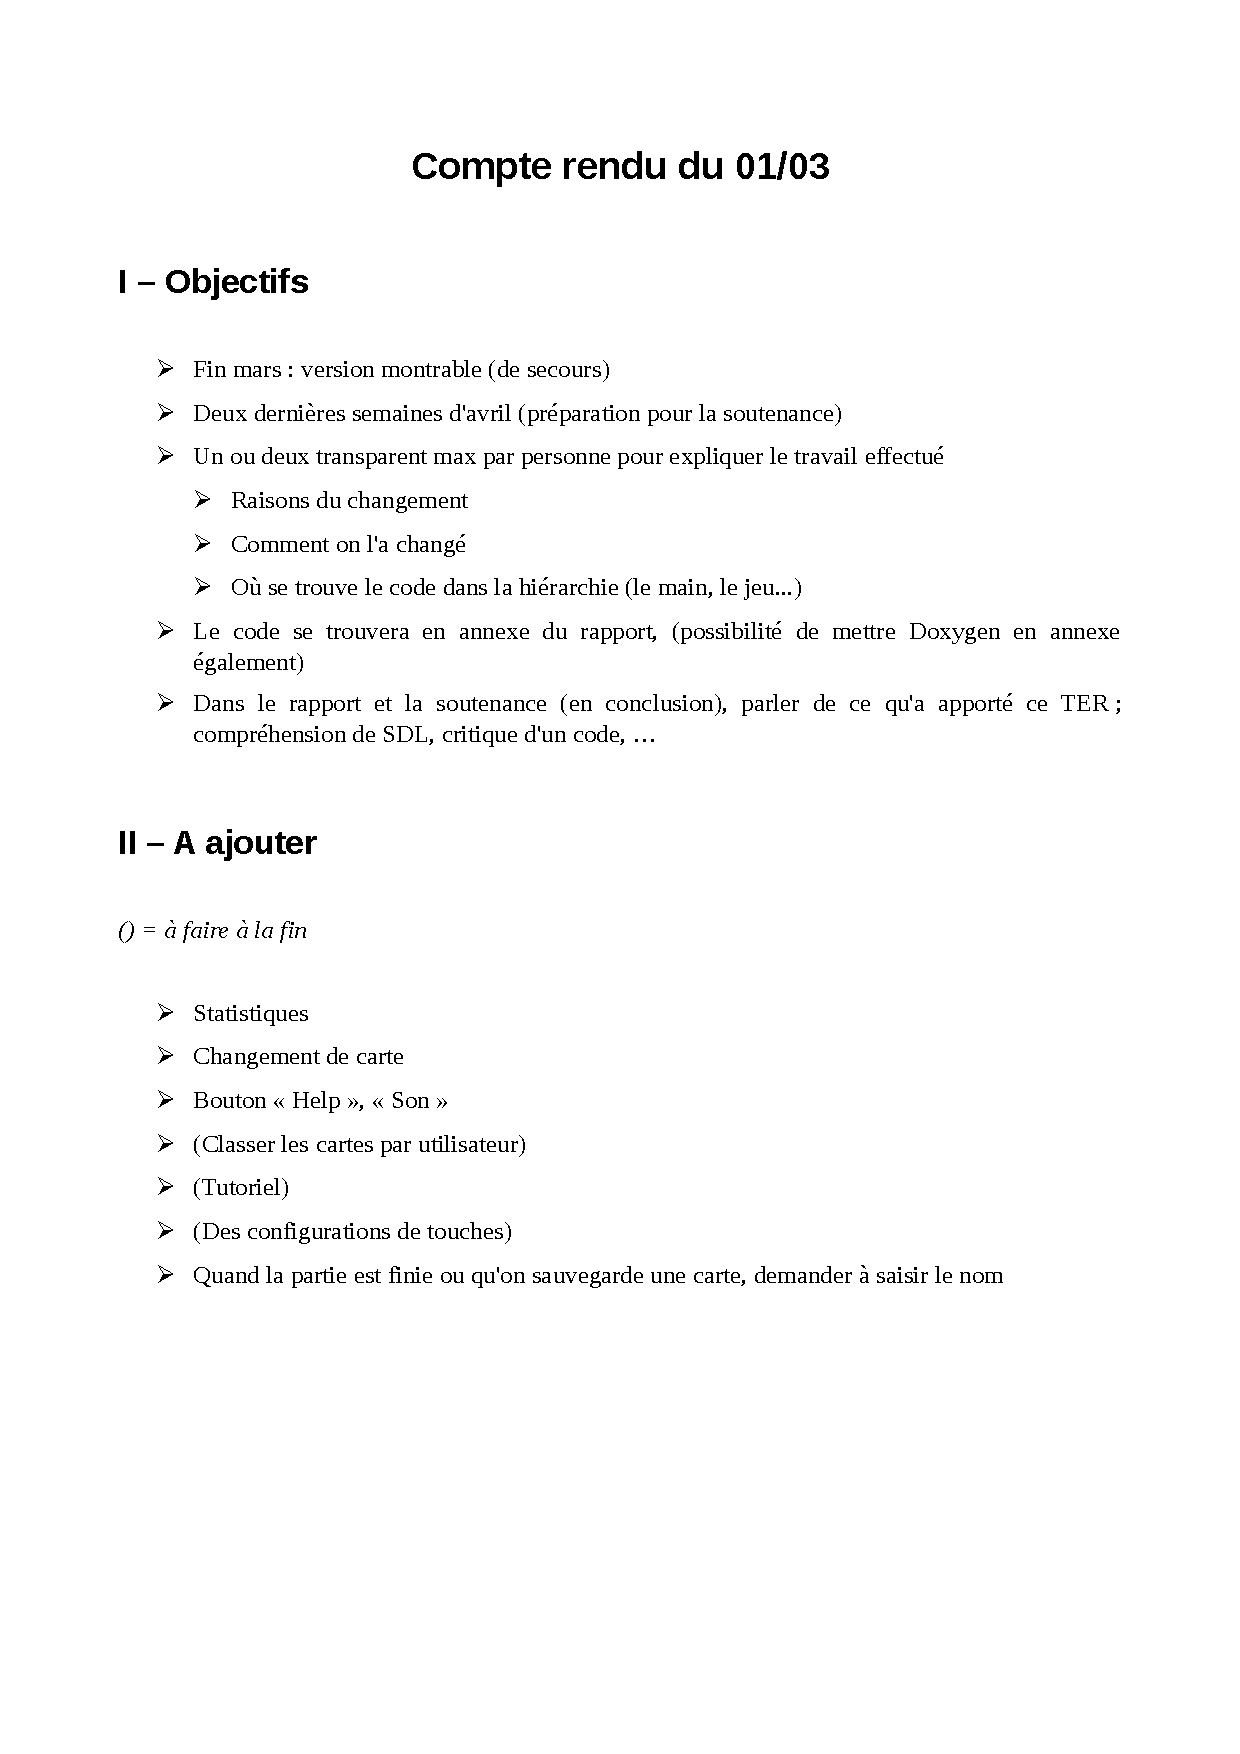
\includepdf[pages={1}]{CR5.pdf}
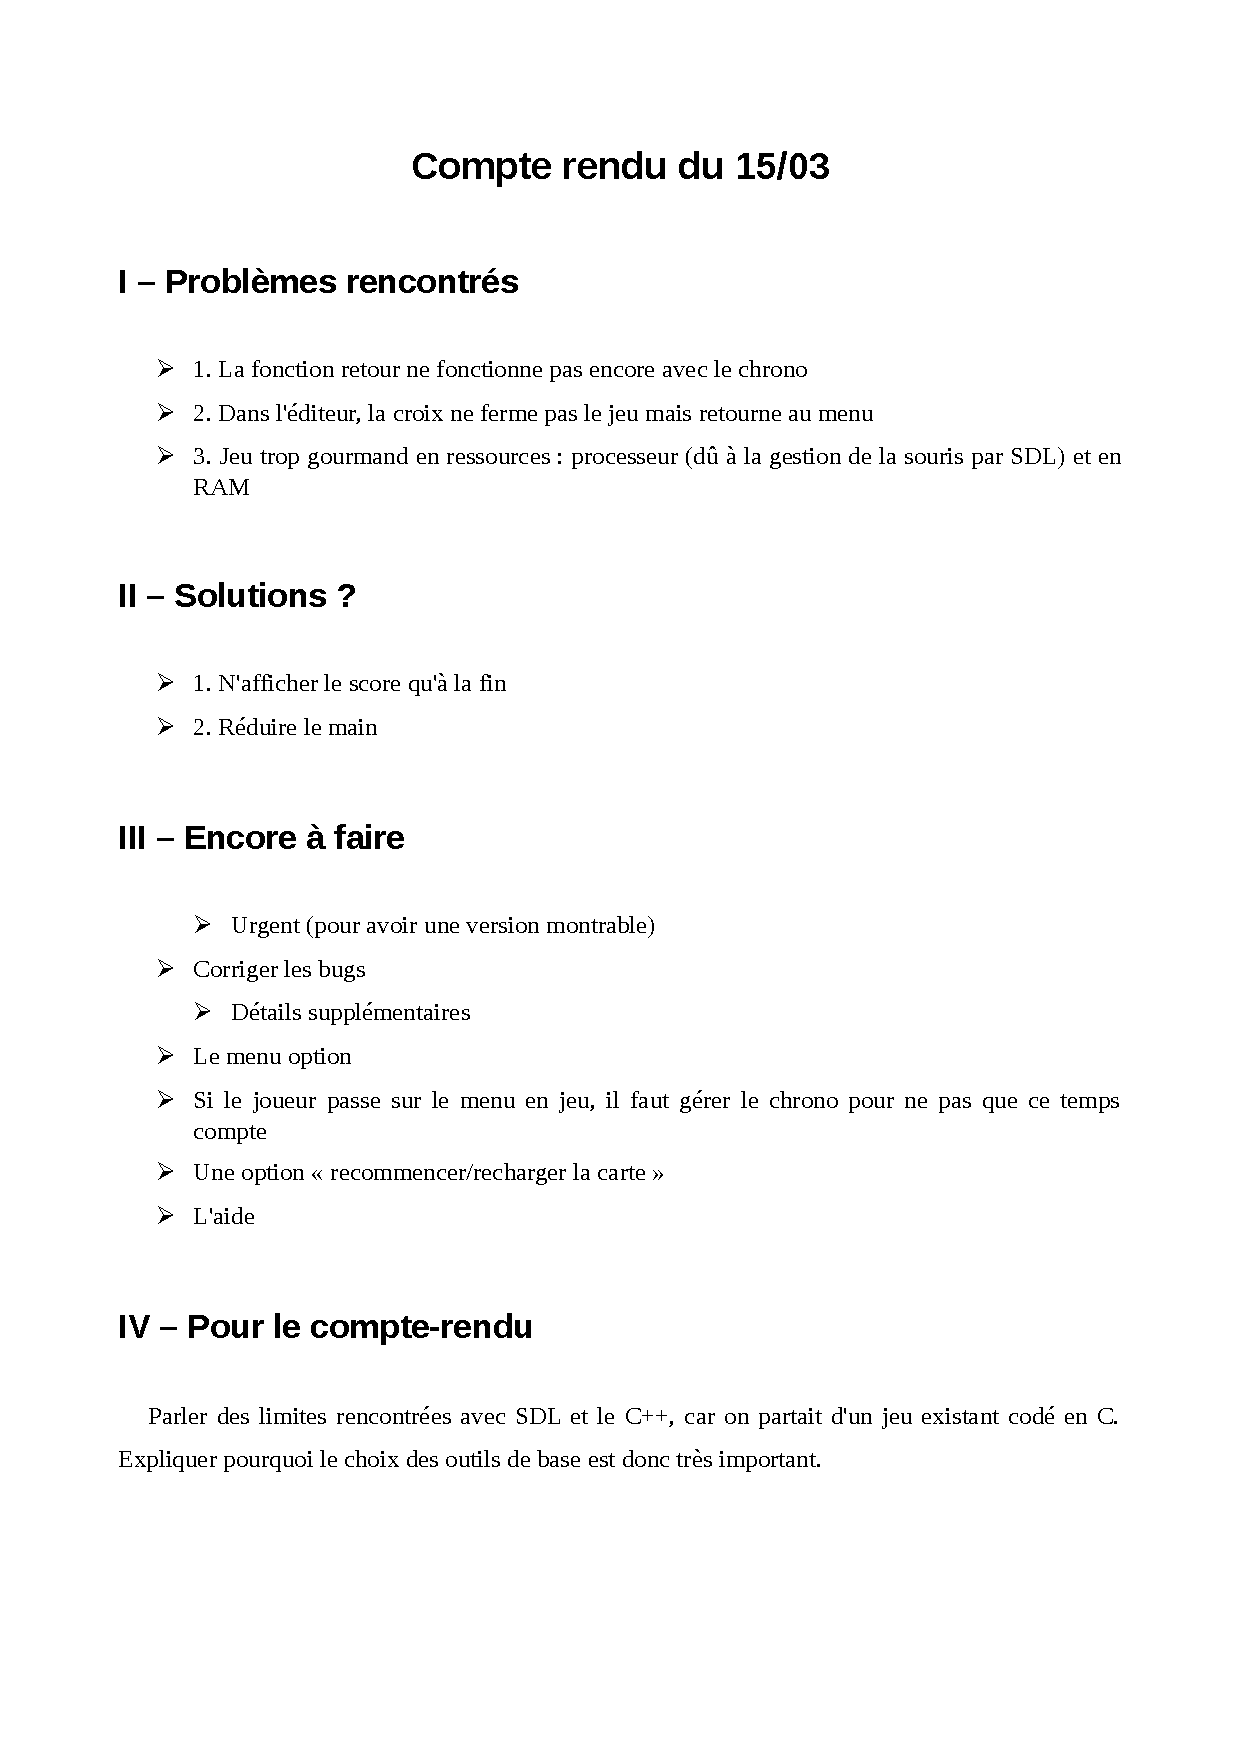
\includepdf[pages={1}]{CR6.pdf}
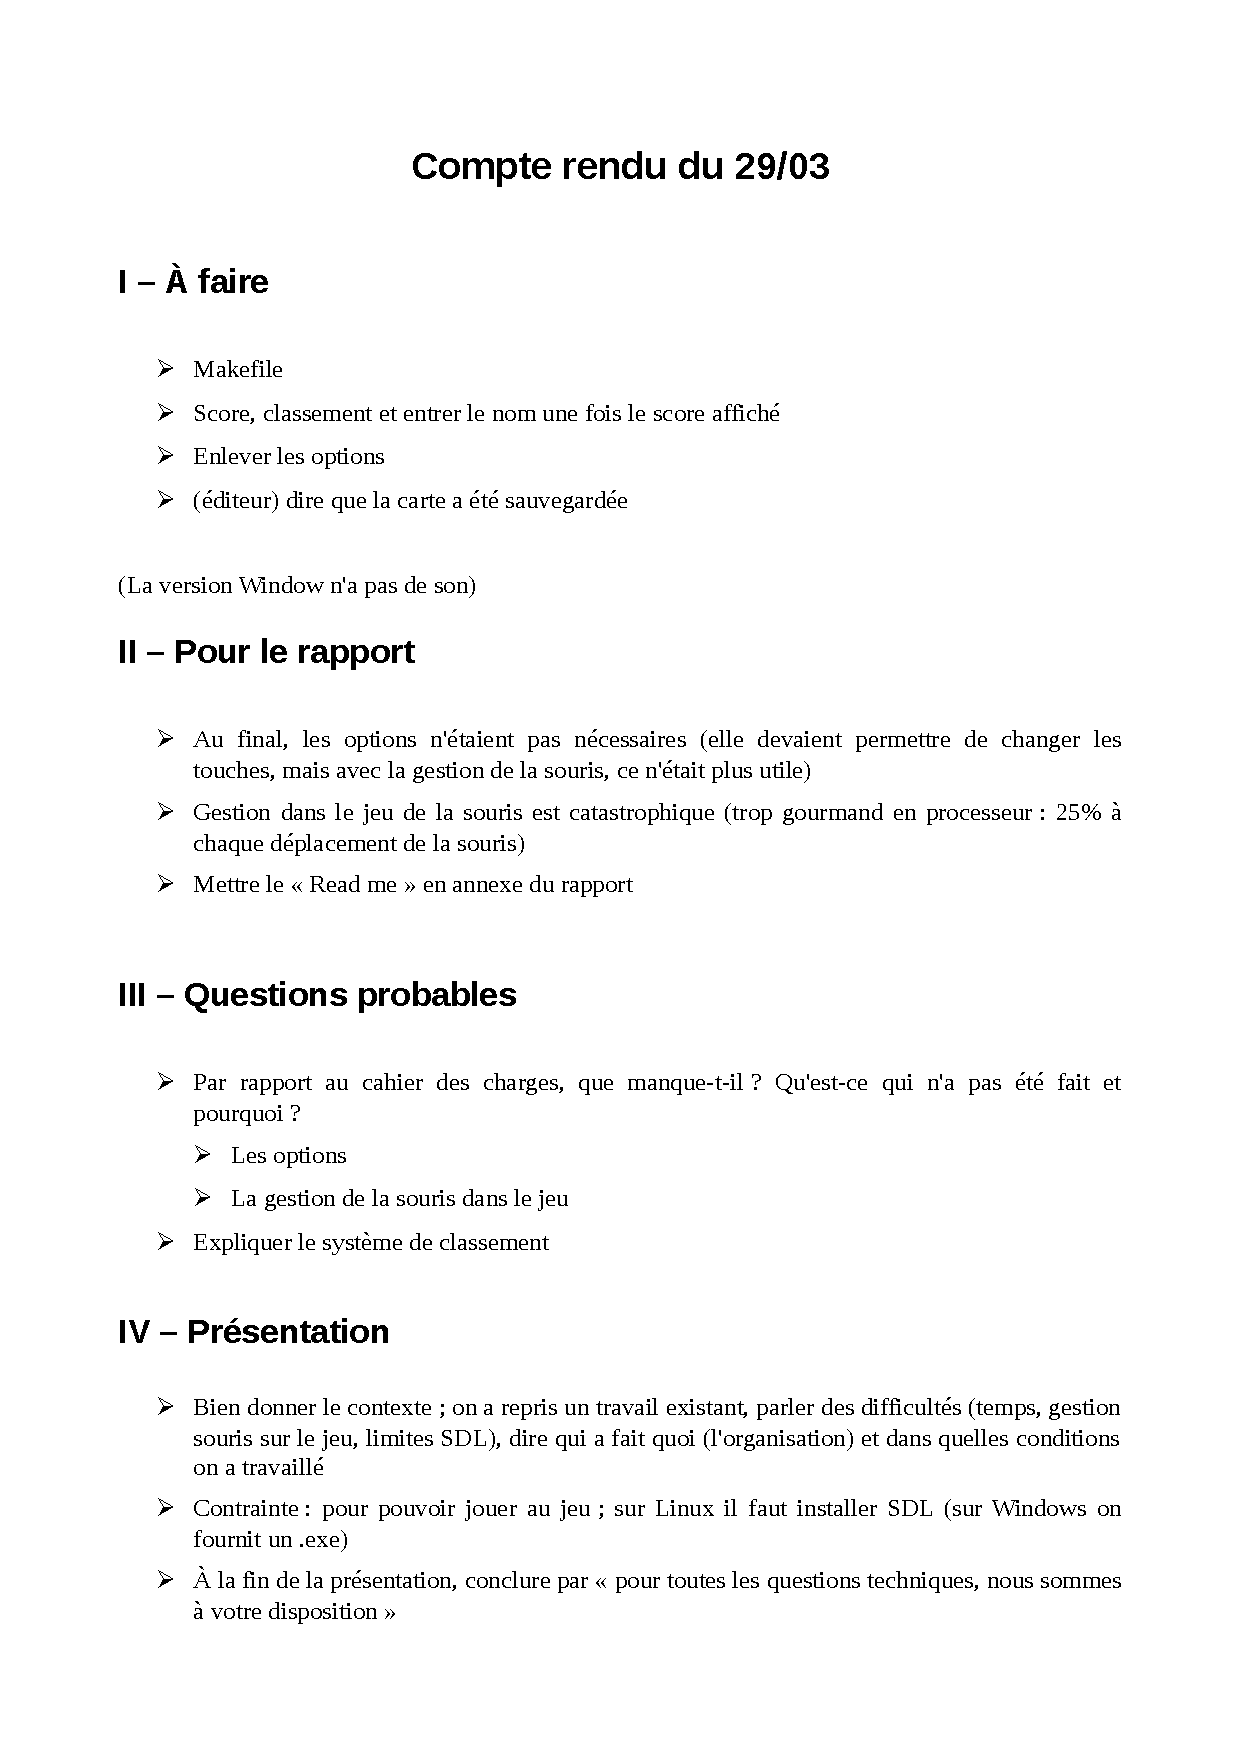
\includepdf[pages={1,2}]{CR7.pdf}

%_____________________________________________________________________________
\chapter*{Conclusion}
%_____________________________________________________________________________

Notre projet consistait à améliorer une version préexistante d’un jeu de réflexion : « mario sokoban »  et ainsi à compléter un travail déjà existant (en langage C que nous avons adapté en langage C++ par la suite).\par
\vspace{0.2cm}
Dans un premier temps, ce projet nous a amené à maîtriser l’utilisation de la bibliothèque « SDL » qui nous était inconnue.  Cette bibliothèque nous a permis de nous initier à la programmation multimédia en 2D, nous a appris à gérer les événements ainsi que l’affichage et la gestion des images, du son, de la souris.\par
\vspace{0.2cm}
Néanmoins nous nous sommes vite rendu compte que cette bibliothèque n'offrait qu'un champ de travail limité, en effet nous avons rencontré beaucoup de problèmes, dont deux principaux. Le premier concernait le processus ; dès lors que nous avons intégré la gestion de la souris, le jeu devenait trop gourmand en ressources. Le deuxième était au niveau de l’assemblage de la fonction retour et du chrono qui se sont révélés difficilement compatibles. Cela nous amène à dire que le choix des outils qui seront utilisés tout le long du projet est une étape primordiale.\par
\vspace{0.2cm}
De plus, il s'agissait ici d'un projet de création d'un jeu en 2D. Si nous sommes un jour amené à créer un autre jeu, nous choisirons certainement un autre environnement.\par
\vspace{0.2cm}
Dans un deuxième temps, ce projet  nous a permis d’approfondir et d’enrichir nos connaissances dans le langage C/C++.\par
\vspace{0.2cm}
Nous estimons qu’à la fin de ce projet, le travail obtenu est satisfaisant dans la mesure où cette version améliorée respecte le cahier des charges qui était fixé, dans la mesure des limites imposées par les conditions de départ (reprendre un travail en C, qui utilisait SDL).\par
\vspace{0.2cm}
Bien entendu, les possibilités d'amélioration ne se limitent à notre travail. Il serait possible de le rendre encore meilleur : en le mettant en ligne, ou à disposition au téléchargement, en ajoutant un multi-joueurs, en programmant des cartes aléatoires qui seraient générées à l’infini...\par
\vspace{0.2cm}
Pour conclure, nous tenions à remercier notre encadrant, Violaine Prince, qui nous a guidés et aidés tout au long du projet.\par
\vspace{0.2cm}

\bibliographystyle{unsrt}
\bibliography{biblio}


\printbibliography


\end{document}